
%(BEGIN_QUESTION)
% Copyright 2006, Tony R. Kuphaldt, released under the Creative Commons Attribution License (v 1.0)
% This means you may do almost anything with this work of mine, so long as you give me proper credit

A flow measurement technique known as {\it twin-turbine} is able to measure the true mass flow rate of a fluid stream, by measuring the angular displacement between two turbines connected together by a torsional spring coupling.  The two turbines have different blade pitches, which means they ``want'' to rotate at different speeds for any given flow rate.

Turbine rotation is detected by a ``pick-up'' coils, one at each turbine.  If spun by hand while the flowmeter was placed on a workbench, the two turbines would of course spin at the same speed with no torque generated between them.  Their respective pulse output waveforms, when viewed with an oscilloscope, should look something like this:

$$\includegraphics[width=15.5cm]{i00533x01.eps}$$

\filbreak

Explain and sketch what the two waveforms would look like if an actual fluid was flowing through the flowmeter body:

$$\includegraphics[width=15.5cm]{i00533x02.eps}$$

\underbar{file i00533}
%(END_QUESTION)





%(BEGIN_ANSWER)

$$\includegraphics[width=15.5cm]{i00533x03.eps}$$

%(END_ANSWER)





%(BEGIN_NOTES)


%INDEX% Measurement, flow: twin-turbine (mass)

%(END_NOTES)


